\documentclass[a4paper,12pt]{article}
\usepackage[utf8]{inputenc}
\usepackage[T1]{fontenc}
\usepackage{graphicx}
\usepackage[french]{babel}
\usepackage{icomma}

\title{Questions adaptatives}
\author{Jill-Jênn Vie}

\begin{document}
\maketitle

\section{Introduction}

Étant donné un utilisateur possédant une capacité $c$ parmi un ensemble $C$, et un ensemble de questions binaires $Q$ dont on connaît pour chaque $q \in Q$ la probabilité que l'utilisateur réponde \emph{oui} sachant que sa capacité est $c \in C$, on s'intéresse à déterminer $c$ le mieux possible en posant un sous-ensemble de questions de $Q$ de manière adaptative : chaque question $q^{(i)}$ est choisie en fonction des réponses aux questions $q^{(1)}, \ldots, q^{(i - 1)}$, à valeurs dans $\pm 1$.

La capacité $c$ peut être connue de l'utilisateur qui pose les questions (auquel cas l'interaction s'apparente à une devinette où le système doit trouver l'objet pensé) ou inconnue (évaluation d'un niveau, sondage préalable à un algorithme de recommandation, test de personnalité).

Ce problème semble être une généralisation de la \emph{théorie de la réponse à l'item}, où le niveau d'un candidat est modélisé par une variable $\theta \in [-5, 5]$ et on connaît la probabilité qu'un candidat réponde correctement à la question $q_i$ sachant qu'il a le niveau $\theta = k$. Il semble également constituer un modèle d'erreur pour le problème de \emph{recherche de contenu par comparaisons} (étant donné un point cible d'un espace $E$, combien de questions de la forme \og la cible est-elle plus proche de $y$ que de $z$ ? \fg{} (où $y, z \in E$) faut-il poser de manière à déterminer la cible avec une probabilité satisfaisante ?).

\section{Modélisation}

On numérote les questions $Q = \{q_1, \ldots, q_m\}$ et les capacités $C = \{c_1, \ldots, c_n\}$ et on considère que la réponse $R_{ij}$ à la question $q_i$ sachant que le sujet a pour capacité $c_j$ est modélisée par une loi bêta de paramètres $(\alpha_{ij}, \beta_{ij})$ :
\[ p(R_{ij} = 1) = \frac{\alpha_{ij}}{\alpha_{ij} + \beta_{ij}}. \]

Ainsi, si $\tilde{R}$ est la matrice d'élément principal $(\alpha_{ij} / (\alpha_{ij} + \beta_{ij}))$, la réduction d'entropie par question est donnée par la relation :
\[ \Delta H = H(\tilde{R}) \pi - H(\tilde{R} \pi) \]

\begin{figure}
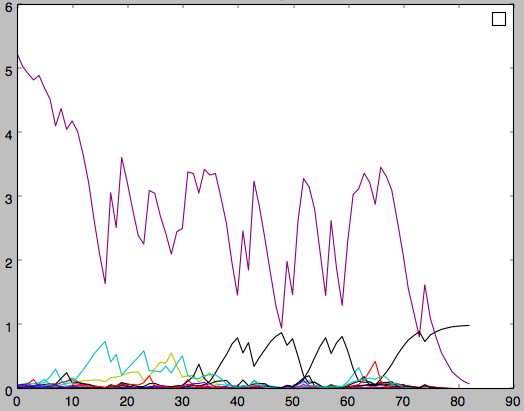
\includegraphics[width=\linewidth]{game.png}
\caption{20 questions, 50 objets.}
\end{figure}

\section{Algorithme}

\noindent
$\pi \leftarrow \textnormal{Uniforme}(n)$\\
Tant que $H(\pi) > 0,1$\\
\indent Poser la question $j$ telle que $j = \textnormal{argmin}_j (\Delta H)_j$\\
\indent Mettre à jour $\pi$ via la formule de Bayes\\
Renvoyer $\pi$

\section{Discussion}

Les questions suivantes retiennent notre attention :
\begin{itemize}
\item Au bout d'un budget de $b$ questions, quelle est l'incertitude sur le résultat (l'entropie moyenne obtenue au bout de $b$ questions) ?
\item Combien faut-il poser de questions pour obtenir une incertitude raisonnable sur la capacité du candidat ?
\item Partant d'une matrice $\widehat{R}$ mise à jour empiriquement, les questions les plus fréquemment posées sont-elles les meilleures (au sens de $\tilde{R}$) ?
\end{itemize}

\end{document}
